\section{Электрофорез}

В данном разделе использовались материалы из методического пособия по генной инженерии.

Электрофорез по Лэммли является одним из наиболее популярных методов по работе с белками. С
помощью электрофореза в полиакриламидном геле, белки можно фракционировать по молекулярной
массе, размерам и форме, так как данный метод имеет большую разрешающею способность. Преимущества
данного метода следующие: гель химически стабилен, нет электроосмоса, устойчивость к
растворителям, изменению рН и температуре.

Процесс полимеризации полиакриламидного геля представляет собой химическую реакцию,
мономером которой служит акриламид. Так как реакция протекает по радикальному механизму, то
в качестве молекулы-инициатора служит персульфат аммония (ПСА). Полимеризация начинается с
образования радикала из ПСА. Катализатором процесса служит тетраметилэтилендиамин (ТЕМЕД). Первая
реакция инициирует разрыв связи между двумя атомами кислорода в молекуле персульфата аммония. В
результате этой реакции образуется свободный радикал с одним неспаренным электроном у атома
кислорода. Данный радикал влияет на разрыв двойной связи в молекуле акриламида. Такая цепная
реакция продолжается, пока два радикала не образуют между собой ковалентную связь.

\subsection{Подготовка белков}

Так как многие белки имеют вторичную, третичную и иногда четвертичную структуру, то следует их
предварительно денатурировать, чтобы избежать влияния структуры и заряда белка на его
подвижность в геле. Для этого их кипятят в Sample Buffer (SB). Это буфер, который включает краситель
бромфеноловый синий (позволяет нам следить за ходом процесса), глицерин (облегчает нанесение
образца на гель), SDS и $\beta$-меркаптоэтанол. SDS -- это ионный детергент (додецилсульфат натрия), который
за счет гидрофобных взаимодействий связывается с белками в соотношении 1,4 мг SDS на 1 мг белка. Так
как в растворе образуется избыток диссоциированных остатков сульфокислоты, собственный заряд
белка становится несущественным. $\beta$-меркаптоэтанол способствует разрыву дисульфидных связей в
молекуле белка. Денатурации белка также способствует кипячение. Из этого можно сделать вывод, что
в полиакриламидном геле разделение белков идет только по массе.

\subsection{Суть процесса}

Одна из особенностей данной системы ЭФ заключается в том, что участвуют 2 геля --
разделяющий (мелкопористый, нижний) и концентрирующий (крупнопористый, верхний). Кроме размеров
пор, эти гели отличаются по pH. В концентрирующем геле разделение белков не происходит. В нем белки
собираются в одну узкую полосу. Для разделяющего геля эта полоса будет стартом для начала
фракционирования. Смысл процесса заключается в следующем: сразу после включения электрического
напряжения, напряженность электрического поля одинакова по всему гелю. Образцы начинают входить
в гель. Ионы глицина в концентрирующем геле имеют отрицательный заряд и начинают замещать ионы
хлора. Следовательно, в концентрирующем геле (с более кислым pH) большинство молекул глицина
изменят заряд на нейтральный. Такая нейтрализация увеличивает напряженность электрического
поля в концентрирующем геле и образцы начнут двигаться. В разделяющем геле можно наблюдать обратное
изменение напряженности поля. Это приведет к замедлению движения белков.
С этого момента начнется медленное разделение белков под воздействием низкой напряженности
электрического поля.


\subsection{Исходные концентрации проб}
После рассмотрения концентраций проб, полученных спектрофотометрическим методом
и методом Брэдфорд, было обнаружено, что точность концентрации пробы 2 вызывает
сомнения.

Значения концентрации пробы 3, полученные обоими методами, почти совпали (6 mg/ml).
Концентрация пробы 1 принята за 15.6 mg/ml.
Концентрация пробы 2 должна быть меньше концентрации пробы 1
(уже потому, что объем, из которого отбиралась проба 1,
меньше объема, из которого отбиралась проба 2).
В то же время, концентрация пробы 2 должна быть больше концентрации пробы 3,
так как проба 3 отбиралась из раствора, из которого была удалена альдолаза.
Учитывая эти соображения, решили грубо округлить концентрацию пробы 2.
Для дальнейших расчетов использовали значение 10.8 mg/ml.

\subsection{Разбавление белковых проб}
Масса, которую можно поместить на дорожку, равна 5 µg.
Объем, помещаемый на дорожку, равен 10 µl.
Следовательно, для использования пробы в электрофорезе концентрация
белка должна быть примерно 0.5 mg/ml.
Объем образца для электрофореза: 200 µl.
Было решено сначала разбавить все пробы в 5 раз, после чего
отобрать из них объем, необходимый для электрофореза.

Чтобы получить образец с концентрацией 0.5 mg/ml,
из раствора, полученного разбавлением пробы в 5 раз,
необходимо отобрать
$$ V = N \frac{C_2 V_2}{C_1} = 5 \frac{0.5 \text{mg/ml} \cdot 0.2 \text{ml}}{C_1} = \frac{0.5}{C_1} \text{[ml]} $$
где $C_1$ -- концентрация белка в пробе.

Рассчитаем объемы, которые нужно отбирать из разбавленных в 5 раз проб:

\begin{tabular}{|c|c|c|}
\hline
Проба & $C_1$ [mg/ml] & $V$ [µl] \\
1 & 15.6  & 32.05 \\
2 & 10.8  & 46.3  \\
3 & 6.2   & 80.65 \\
4 & 32.7  & 18.7  \\
\hline
\end{tabular}

\subsection{Приготовление образцов для электрофореза}
4-х кратный буфер для образцов (SB) был выдан преподавателем.
Для получения однократного буфера, 4-х кратных буфер был разбавлен в 4 раза.
В 1 мл SB было добавлено 50 µl меркаптоэтанола,
концентрация меркаптоэтанола в полученном буфере 5\%.
Для получения образцов для электрофореза сначала добавляли воду,
затем пробу белка, разведенную в 5 раз, затем 50 µl SB.

\begin{tabular}{|c|c|c|c|}
\hline
Проба & \ce{H20} & Проба/5 & SB \\
1 & 118 & 32   & 50 \\
2 & 104 & 46   & 50 \\
3 &  70 & 80   & 50 \\
4 & 131 & 18.7 & 50 \\
\hline
\end{tabular}

\subsection{Маркеры для электрофореза}
\begin{enumerate}
\item Phosphorilase B, 97 kDa
\item BSA, 66.2 kDa
\item Ovalbumin, 45 kDa
\item Carbonie anhydrase, 31 kDa
\item Trypsin inhibitor, 21.5 kDa
\item Lysozime, 14.4 kDa
\end{enumerate}
Оптимум нанесения: 3--5 µl на дорожку.
Хранение при -20\celsius.

\subsection{Проведение электрофореза}
\label{ef}
В 10 лунок геля были нанесены образцы:
\begin{enumerate}
\item маркер
\item проба 1 (8 µl, 4 µg)
\item проба 2 (8 µl, 4 µg)
\item проба 3 (8 µl, 4 µg)
\item проба 4 (8 µl, 4 µg)
\item пустая
\item проба 1 (16 µl, 8 µg)
\item проба 2 (16 µl, 8 µg)
\item проба 3 (16 µl, 8 µg)
\item проба 4 (16 µl, 8 µg)
\end{enumerate}

Параметры электрофореза: 20 mA, 400 V.

\subsection{Результаты электрофореза}
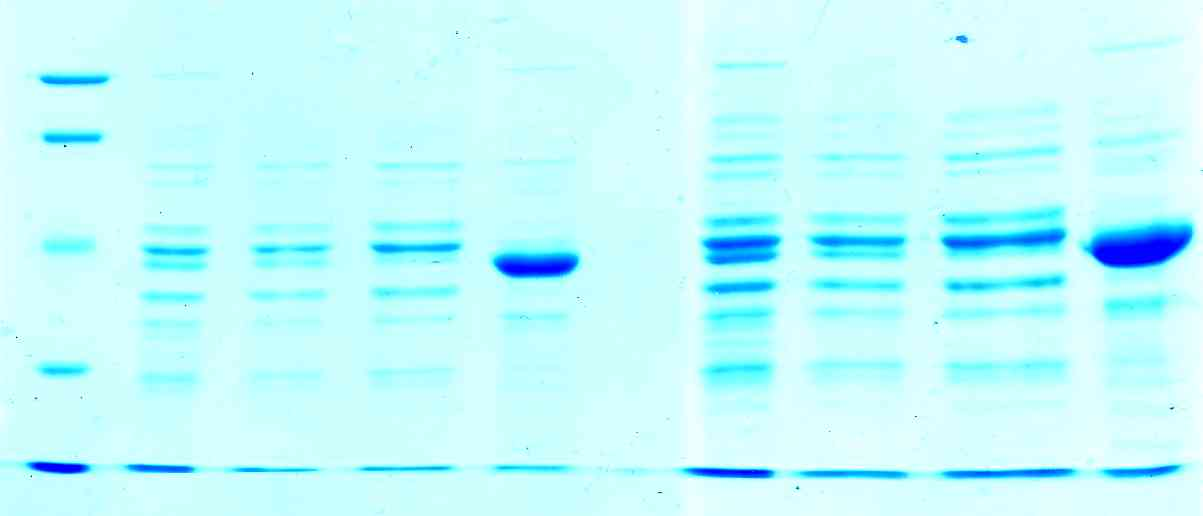
\includegraphics[width=\linewidth]{ef.jpg}

\emph{Вывод}: последняя стадия эффективно отделила альдолазу.

К сожалению, белки-маркеры оказались подпорченными,
в связи с чем оценить массу выделенного белка не удалось.

